\section{System Design}

Our adaptive remastering mechanism is based on the CalvinFS~\cite{thomson2015calvinfs} system. CalvinFS leverages the features of Calvin, which avoids ordering operations when holding the locks to manage metadata storage for file system. However, low throughput stemmed from the long RTT between geo-distributed replicas requires us to adjust the system architecture to trim the cross-replica communication. In general, the key insight is that we assign each file with a local master replica to manage the read/write operations of this file, and transactions involved with only locally-mastered metadata will be serialized locally, without a cross-replica Paxos application to achieve global ordering. Hereby, we name our modified CalvinFS system as \name.

\subsection{System Components}
\name{} consists of following key components, \textsf{Scheduler}, \textsf{BlockLog}, \textsf{MetaStore}, \textsf{PaxosApp}, and \textsf{BlockStore}. As shown in Figure~\ref{fig:arch}, clients submit requests to \textsf{BlockLog}, which parses the transactions and distribute them to corresponding machines. Then it submits a batch of transactions to \textsf{PaxosApp} for ordering. \textsf{Scheduler} on each machine will fetch the output sequence of all transactions from the \textsf{PaxosApp} in local replica, and then call the \textsf{MetaStore} to execute the the transaction. In the following, we will delve into details about \textsf{Scheduler}, \textsf{BlockLog}, and \textsf{PaxosApp}, which carries the essential logic of CalvinFS.

\begin{figure*}[tp]
\centering
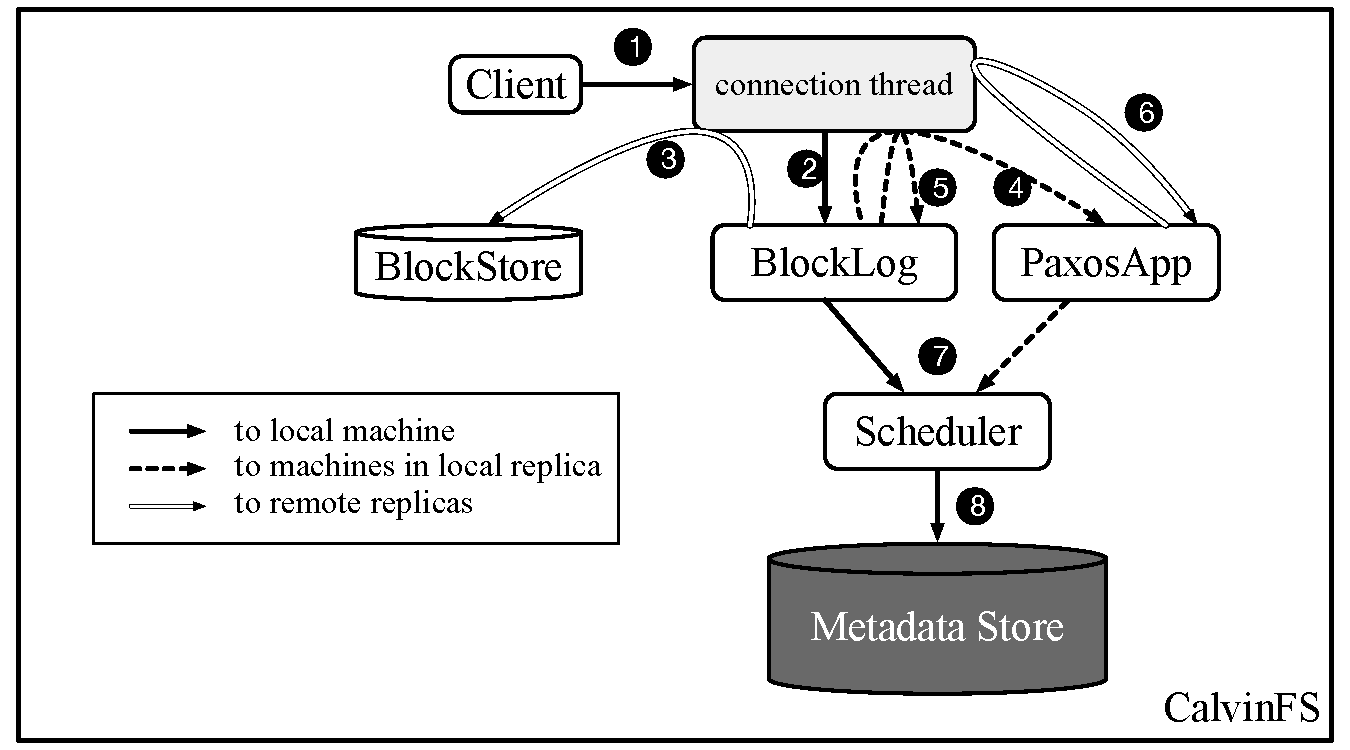
\includegraphics[width=1.8\columnwidth]{figures/arch}
\caption{Logical components of the CalvinFS and the interactions between them}
\label{fig:arch}
\end{figure*}

\heading{BlockLog} 

\noindent This module lies in the center of the \name{}. It interacts with clients, the scheduler, and the sequencer. Client will submit requests to the BlockLog application on the same machine. And, BlockLog will periodically pop all the pending requests in the queue, gather them into a batch, and send the batch to each replica for durability. After that, it will submit the batch ID to PaxosApp for a global sequence, because each machine concurrently receive and process requests from clients. BlockLog also interacts with the Scheduler module by exposing the interface where PaxosApp outputs the batch ID sequence to it.

\heading{Scheduler}

\noindent This module controls when a certain transaction will be executed by the Metastore, so as to guarantee the isolation property. It will first fetch the output sequence from the PaxosApp, and then tries to acquire locks from the readset and writeset of the transaction. Unlike common 2PL protocol, there is a deterministic order before processing the transaction, thus there is no need to release the lock when it is occupied by other ongoing transactions. After acquiring all locks, the Scheduler will call the MetaStore to execute the transaction asynchronously.

\heading{PaxosApp} 

\noindent In traditional CalvinFS, PaxosApp runs on only one machine in each replica, and all requests received by all the machines will be sent to the PaxosApp in their local replica. And, there is a simple Paxos protocol running among all participants from all replicas. To reduce the latency caused by cross-replica communication in Paxos protocol, metadata could be further partitioned into different parts, each of which is assigned to a local replica to manage. In this case, aside from serialize locally submitted requests, PaxosApp also has to coordinate with remote participants to realize the sequence of transactions belonging to other replicas. 




All aforementioned modules are located on each machine within each replica, and each module is registered as an application, running as an independent thread, and communicate with each other through a common communication thread (in each machine), which will further dispatch the messages to corresponding message handling thread to execute.

\subsection{Remaster Protocol}

\begin{figure}[tp]
\centering
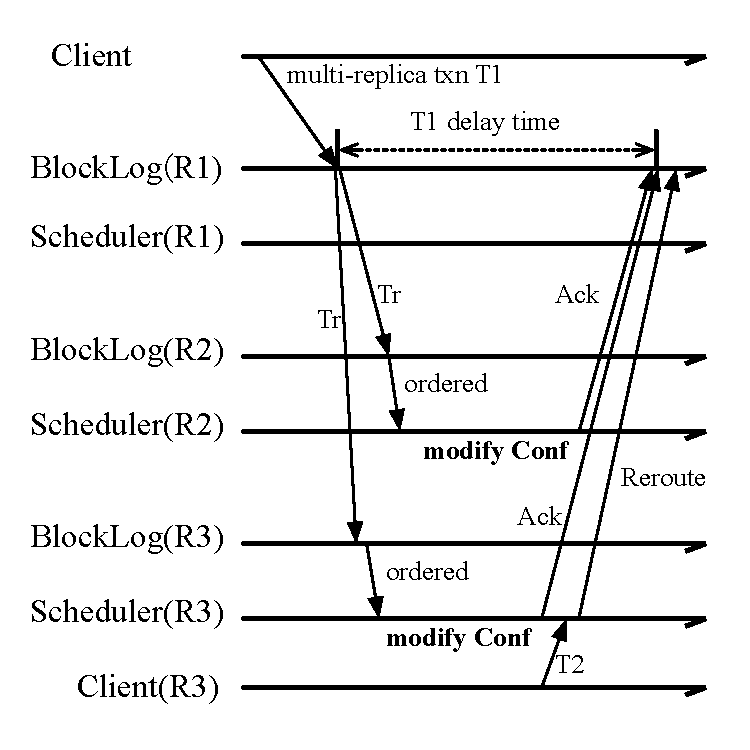
\includegraphics[width=\columnwidth]{figures/flow}
\caption{Explanation of how does Remaster protocol proceed when a distributed transaction T1 arrives}
\label{fig:flow}
\end{figure}

Previous transaction processing logic works well when the static partition of metadata perfectly matches the file access pattern where no distributed transaction appears. However, when there exists distributed transaction, realizing the order the transaction from other replicas will take at least 1 RTT, which means the local replica has to first acquires all locks and then wait at least 1 RTT before proceeding. This waiting time is large enough to impede the throughput of the system. On the other hand, it is extremely hard, if not impossible to achieve the perfect partitioning, not mention such partitioning could become unfit when time goes. Following this basic idea, we further extend static partitioning into an adaptive algorithm, which is called remaster, the master of each file is not statically decided but rather dynamically switched between replicas. In the following, we will introduce how we modify the logic of BlockLog and Scheduler so as to support remaster and as well the \name{} system.

Figure~\ref{fig:flow} illustrates the logic flow of the remaster protocol, and we will delve into details explaining how BlockLog and Scheduler modules work.

\subsubsection{BlockLog Logic}
In \name{}, each multi-replica transaction will incur an adjustment of the master replica assignment for those involved directory. Therefore, BlockLog will first check whether a transaction is multi-replica distributed transaction. If it is a multi-replica transaction, instead of creating a batch, BlockLog will pause this transaction in a specific waiting queue, and then it will create a special transaction, namely remastering transaction $T_r$, to all participating remote replicas, which will further modify their configuration when receiving such transaction, to note the change of the master for this directory.

We also add two additional message handling methods in BlockLog, reroute and remaster\_ack, respectively. When the remote replicas successfully change their configuration, they need to let the primary replica know it is legible to release waiting transaction to proceed as a local transaction in primary replica. Therefore, they send a remaster\_ack message to the BlockLog in primary replica, which will modify the configuration file of the primary replica and further selects those legible pending multi-replica transactions to create batch and begin running as a local transaction. Reroute method deals with the inconsistent views. When a transaction is falsely sent to a replica where it should not be executed, then once the Scheduler realize, it will call reroute method to resend the transaction to the right position.

\subsubsection{Scheduler Logic}
The Scheduler has to deal with the remaster transactions. When the remote replica's scheduler receives a batch of transaction, then for each transaction in it, it has to first verify whether it is a normal single-replica transaction, or it is a falsely sent transaction, or it is a remaster transaction which modify the configuration. The scheduler distinguishes the three cases by the keywords in transaction packet, including the original replica where it is received, and the remaster operation notifier. After realizing the status of the transaction, it will modify the configuration file if it is a remaster transaction; send a reroute RPC call to BlockLog if it is a falsely sent transaction; and acquire lock to execute the transaction if it is a normal single-replica transaction.







